\newpage
\subsection{Verification of welded joints subject to static loading}
	
	\paragraph{Problem} Verify the structural integrity of welds 1 (full penetration butt-welded joint), 2 (fillet-welded joint) and 3 (full penetration welded joint) of the support arm made up of \texttt{S235} and shown in figure \ref{ex:welddraw}. For the problem consider $P = 10kN$, $L=2\,000mm$, $H=250mm$, $h = 5mm$, $S_p = 5mm$, $\sall = 160 MPa$, $\nu= 0.85$, $\nu_1 = 0.7$, $\nu_2= 0.85$.
	
	
	\begin{figure}[bht]
		\centering 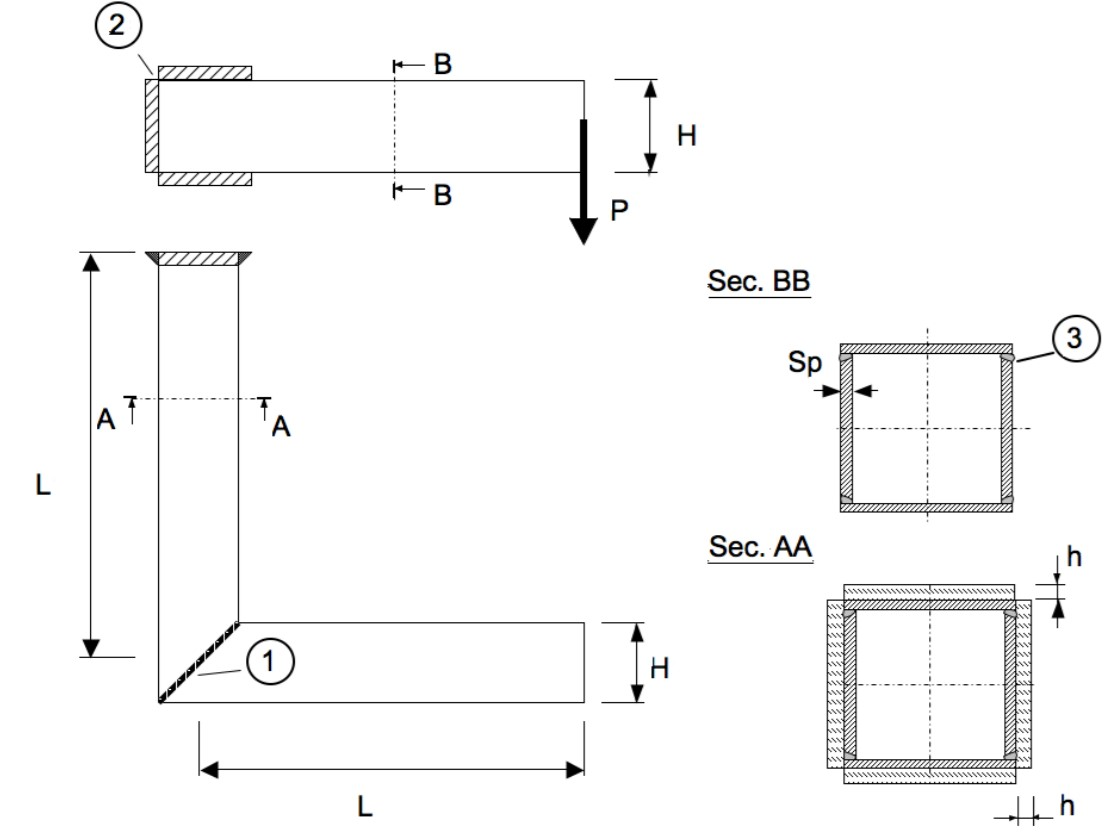
\includegraphics[width=11cm]{ex-weld}
		\caption{sketch of the structure with welds that has to be verified.} \label{ex:welddraw}
	\end{figure}
	
	\paragraph{Solution}
\begin{enumerate}
	\item for the full penetration weld we have to consider figure \ref{ex:weld1}; respect to the drawn section we have a vertical (toward $z$) shearing force $V = P= 10\,000N$ that produces a bending $M_{b,y}$ (toward $y$ axis) and torsional $M_{t,x}$ moments as:
	\[ M_{b,y} =  PL \cos 45^\circ = 1.41\cdot 10^7 N \cdot mm \hspace{2cm} M_{t,x} = - PL \cos 45^\circ = -1.41\cdot 10^7 N \cdot mm  \]
	
	\begin{SCfigure}[1.5][bht]
		\centering 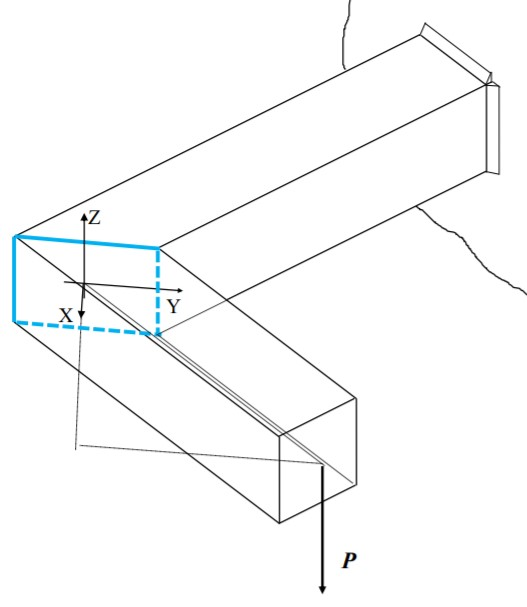
\includegraphics[width=5cm]{ex-weld-1} 
		\caption{full penetration joint and related axis system in order to verify the weld.}
		\label{ex:weld1}
	\end{SCfigure}
	
	Respect to the highlighted area of the weld, the geometric properties are
	\begin{align*}
		I_y & = \frac{H^3 H \sqrt 2}{12} - \frac{(H-2S_p)^3(H-2S_p)\sqrt 2}{12} = 6.94 \cdot 10^7 mm ^4 \hspace{2cm} \\ \Omega & = (H - S_p)(H-S_p)\sqrt 2 = 8.94 \cdot 10^4 mm^2
	\end{align*}
	The bending moment determines an orthogonal normal stress evaluated as
	\[ \sigma_\perp = \frac{M_{b,y}}{I_y} \frac H 2 = 25.4MPa \]
	The torsional moment produces instead a parallel shear stress $\tau_{T}$ that's different for vertical and horizontal beads of welding that, using Bredt's formula, is
	\[ \tau_{T,\textrm{horizontal}} = \frac{M_{t,x}}{2 \Omega S_p} = 16.61MPa \hspace{2cm} \tau_{T,\textrm{vertical}} = \frac{M_{t,x}}{2 \Omega \sqrt 2 S_p} = 11.75MPa  \]
	Considering the stress distribution shown in figure \ref{ex:weld1stress}, the shear load $V$ determines a parallel shear stress $\tau_V$ that majorly adds up with the one due to torsion at the point $A$: using the Jourawsky method we have that
	\[ \tau_{V,A} = V \frac{\frac{H-S_p}{2} \frac{\sqrt 2 H}{2} S_p}{I_y S_p} = 3.12 MPa \qquad \Rightarrow \quad \tau_{max} = \tau_{T,h} + \tau_{V,A} = 19.73MPa \]
	
	\begin{SCfigure}[1][bht]
		\centering 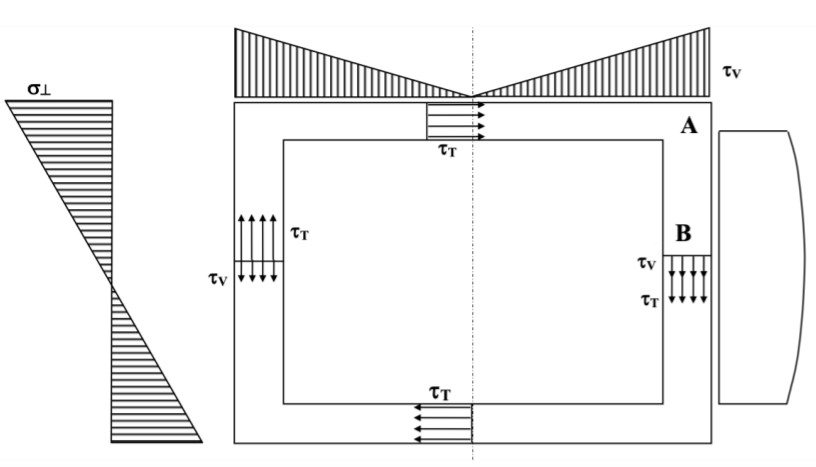
\includegraphics[width=7cm]{ex-weld-1stresses}
		\caption{stress distribution in the cross-section.} \label{ex:weld1stress}
	\end{SCfigure}
	
	Using Von Mises criterion we have an equivalent stress $\seq = \sqrt{\sigma_\parallel^2 + 3 \tau_{max}^2} = 42.58 MPa$; considering as the allowable stress $\sigma_{w,all}$ on the weld as lowered by the weakening factor $\nu$ we have the safety factor as
	\[ \phi = \frac{\sigma_{w,all}}{\seq} = \frac{\nu \sall}{\seq} = 3.19 \]
	
	\item considering now the fillet-welded joint (figure \ref{ex:weld2}) the transmitted load are expressed by
	\[ V = P = 10\,000N \qquad M_x = - PL = -2\cdot 10^7 N\cdot mm \qquad M_y = PL = 2 \cdot 10^7 N\cdot mm\]
	
	\begin{figure}[b]
		\centering 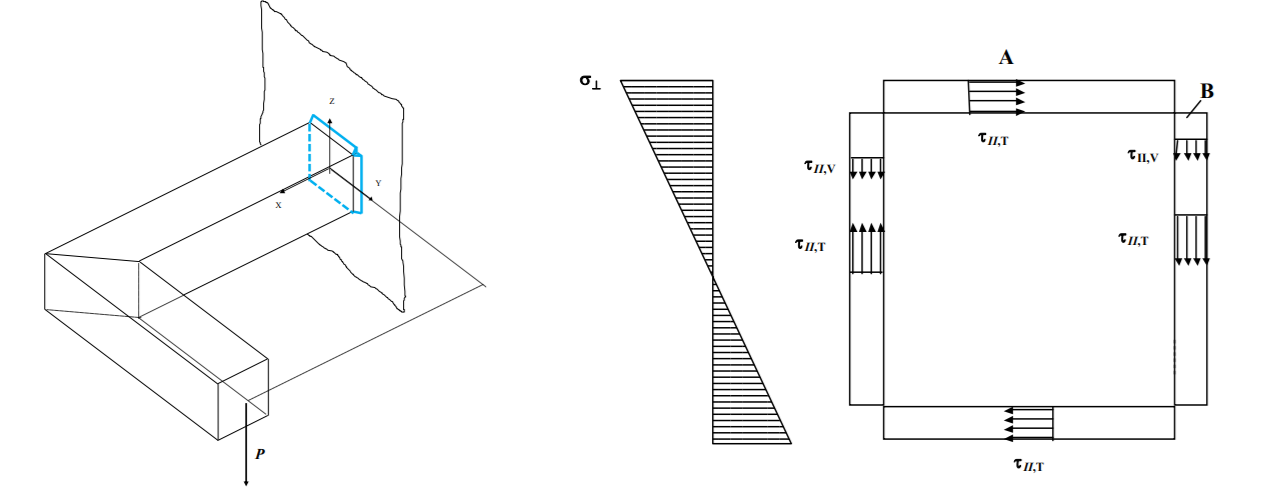
\includegraphics[width=13cm]{ex-weld-2} 
		\caption{fillet-welded joint and related axis system (left) and stress distribution in the overturned cross section (right).} \label{ex:weld2}
	\end{figure}
	
	Considering now the geometric properties of the weld beads we have that the throat height is equal to $ a = h \frac{\sqrt 2}{2} = 3.535mm$ determining an overall throat area $A = 4 A_i = 4 aH = 3.535\cdot 10^3mm^2$; overturning the throat section toward the frame (to simply the calculation) we have a moment of inertia of the section equals to
	\[ I_y = 2 \left(\frac{H+a}{2}\right)^2 a H + 2 \frac{a^3H}{12} + 2 \frac{H^3 a}{12} = 3.76 \cdot 10^7 mm^4  \]
	With that we can compute the maximum orthogonal normal stress $\sigma_\perp$ due to the bending $M_y$ and the parallel shear stress $\tau_T$ due to torsion according to the simplified approach of the force couples:
	\[ \sigma_\perp = \frac{M_y}{I_y} \frac{H+2a}{2} 68.4MPa \hspace{2cm} \tau_T = \frac{M_x}{2 A_i (H+a)} = 44.63 MPa \]
	Assuming that the transverse shear is bore only by the vertical weld beads with a value $\tau_V= \frac{V}{2 A_i} = 5.65 MPa$. Respect to figure \ref{ex:weld2} the verification can be performed in two critical section:
	\begin{itemize}
		\item at the point $A$ we have $\sigma_\perp = 68.4 MPa$ and $\tau= 44.63MPa$ whose equivalent stress is $\seq = \sqrt{\sigma_\perp^2 + \tau^2} = 81.67 MPa$; considering so
		\[ \phi = \frac{\sigma_{w,all}}{\seq} = \frac{\nu_1 \sall}{\seq} = 1.37 \]
		that's an acceptable value for static loading; it's also verified that $|\sigma_\perp| \leq \nu_2 \sall$.
		\item at point $B$ the normal component $\sigma_\perp$ is lowered to the value
		\[ \sigma_\perp = \frac{M_y}{I_y} \frac H 2 = 66.49 MPa \]
		while the tangential component is the sum $\tau = \tau_T + \tau_V= 50.28 MPa$ and so the equivalent stress is $\seq = \sqrt{\sigma_\perp^2 + \tau^2} = 83.36 MPa$ determining a safety factor
		\[ \phi = \frac{\sigma_{w,all}}{\seq} = \frac{\nu_1 \sall}{\seq} = 1.34 \]
		Also in this case is verified the inequality $|\sigma_\perp| \leq \nu_2 \sall$.
	\end{itemize}
	
	\item lastly the welded plates to fabricate the closed section are evaluated at the most stresses location corresponding at the fixed constrained region (where $V = 10\,000N$, $M_{x} = M_y = 2\cdot 10^7N\cdot mm$ ); considering section BB (figure \ref{ex:welddraw}) as representative of the beam, we have the following section parameters:
	\[ \Omega = \big(H-S_p\big)^2 = 60\,025 mm^2 \hspace{2cm} I_y = \frac{H^4}{12} - \frac{(H-S_p)^2}{12} = 4.904 \cdot 10^7 mm^4 \]
	
	We can so evaluate the stress at the weld considering the bending and the torsion as
	\[ \sigma_\perp = \frac{M_y}{I_y} \frac H 2 = 50.98 MPa \hspace{2cm} \tau_T = \frac{M_x}{2\Omega S_p} = 33.31 MPa \]
	Transverse shear stress can be instead estimate by the Jourawsky formula at the location of the joint as
	\[ \tau_V = \frac{P \, H S_p \frac{H-S_p}{2}}{I_y 2 S_p} = 3.12 MPa \]
	Considering the overall $\tau = \tau_T+\tau_V = 36.43MPa$ we have an equivalent stress state (according to Von Mises) of $\seq = \sqrt{\sigma_\parallel^2 + 3\tau^2} = 81.12 MPa$: this allows to verify the structure as
	\[ \phi = \frac{\nu \sall}{\seq} = 1.68 \]
	
	
	
	
	
\end{enumerate}
	
	
	
	
	
	
	
	
	
	
	
	
	
	
	
	
	
	
	
	
	
	
	
	
	
	
	
	
	
	
	
	
	